\documentclass[aspectratio=169]{beamer}

\usepackage{beamerthemesplit}
\usepackage{amsmath}
\usepackage{amsfonts}
\usepackage{amssymb}
\usepackage{cancel}
\usepackage{bussproofs}
\usepackage{graphicx}
\usepackage{minted}
\usepackage{comment}
\usepackage{unicode-math}
\setmathfont{Stix Two Math}
\usepackage[pdf]{graphviz}

% For highlighting MeTTa code
\usepackage{listings}
\usepackage{color}
\definecolor{mygreen}{rgb}{0,0.6,0}
\definecolor{mymauve}{rgb}{0.58,0,0.82}
\definecolor{dgreen}{rgb}{0,0.5,0}
\definecolor{dblue}{rgb}{0,0,0.5}
\definecolor{dred}{rgb}{0.5,0,0}
\lstset{ %
  backgroundcolor=\color{white},   % choose the background color
  basicstyle=\tiny,                % size of fonts used for the code
  breaklines=true,                 % automatic line breaking only at whitespace
  captionpos=b,                    % sets the caption-position to bottom
  commentstyle=\color{mygreen},    % comment style
  escapeinside={\%*}{*)},          % if you want to add LaTeX within your code
  keywordstyle=\color{blue},       % keyword style
  stringstyle=\color{mymauve},     % string literal style
}

\makeatletter
\newcommand{\tinier}{\@setfontsize{\srcsize}{3.5pt}{3.5pt}}
\makeatother

\makeatletter
\newcommand{\tiniest}{\@setfontsize{\srcsize}{2pt}{2pt}}
\makeatother

\mode<presentation>
{
  \usetheme{AnnArbor}
  \usecolortheme{crane}
}

\usepackage[english]{babel}
%% \usepackage[latin1]{inputenc}
\usepackage{times}
\usepackage[T1]{fontenc}

\newcommand{\limp}{\Rightarrow}
\newcommand{\TheoryT}{\texttt{Theory}}
\newcommand{\ProofT}{\texttt{Proof}}
\newcommand{\PropositionT}{\texttt{Proposition}}
\newcommand{\BoolT}{\texttt{Bool}}
\newcommand{\True}{\texttt{True}}
\newcommand{\False}{\texttt{False}}
\newcommand{\axone}{\texttt{ax-1}}
\newcommand{\axtwo}{\texttt{ax-2}}
\newcommand{\axthree}{\texttt{ax-3}}
\newcommand{\axmp}{\texttt{ax-mp}}
\newcommand{\STV}[2]{<\!#1, #2\!>}
\newcommand{\Induction}{Ind}
\newcommand{\Revision}{Rev}

\title{Estimating the Probability of a Conjecture to be a Theorem in PLN for Inference Control}

\author{Nil Geisweiller}

\institute[SingularityNET]
{
  \begin{center}
    
\includegraphics[scale=0.2]{figs/snet-logo.png}\\[1cm]
    Artificial Intelligence and Theorem Proving 2025 (AITP-25)
  \end{center}
}

\date[AITP-25]

\begin{document}

\lstset{language=Lisp}

\begin{frame}
  \maketitle
\end{frame}

\begin{frame}
  Ternary predicate relating theories, proofs and propositions:
  $$\Theta : {\color{violet}\TheoryT} \times {\color{blue}\ProofT} \times {\color{red}\PropositionT} \to \BoolT$$

  \begin{itemize}
  \item {\color{violet}$\TheoryT$}: \emph{Typing relationships} encoding axioms and
    inference rules.
    {\color{violet}$$\{\texttt{Z}:\texttt{Nat},\ \texttt{S}:\texttt{Nat} \texttt{->} \texttt{Nat}\}$$}
  \item {\color{blue}$\ProofT$}: \emph{Inhabitant} of a type.
    {\color{blue}$$\texttt{(S (S (S Z)))}$$}
  \item {\color{red}$\PropositionT$}: \emph{Type}.
    {\color{red}$$\texttt{Nat}$$}
  \end{itemize}
  $$\Theta({\color{violet}\{\texttt{Z}:\texttt{Nat},\ \texttt{S}:\texttt{Nat}
  \texttt{->} \texttt{Nat}\}}, {\color{blue}\texttt{(S (S (S Z)))}}, {\color{red}\texttt{Nat}})
  = \True$$
\end{frame}

\begin{frame}[fragile]
  \frametitle{Example (Propositional Calculus):}
  $
  \begin{array}{lll}
  \Theta & ( & {\color{violet}\{\ } \\
  & & \ \ \ {\color{violet} \axone \ :\ (\phi\ \to\ (\psi\ \to\ \phi)),} \\
  & & \ \ \ {\color{violet}\axtwo \ :\ ((\phi\ \to\ (\psi\ \to\ \chi))\ \to\ ((\phi\ \to\ \psi)\ \to\ (\phi\ \to\ \chi))),} \\
  & & \ \ \ {\color{violet}\axthree \ :\ (((\neg\ \phi)\ \to\ (\neg\ \psi))\ \to\ (\psi\ \to\ \phi)),} \\
  & & \ \ \ {\color{violet}\axmp \ :\ \phi\ \texttt{->}\ (\phi\ \to\ \psi)\ \texttt{->}\ \psi}
  \\
  & & {\color{violet} \} }, \\
  & &
  {\color{blue}
    (\lambda\ (\texttt{mp2.1}\ :\ \phi)\ (\texttt{mp2.3}\ :\ (\phi\ \to\ (\psi\ \to\ \chi)))\ (\axmp\ \texttt{mp2.1}\ \texttt{mp2.3}))
    },
  \\
  & &
  {\color{red}
    \phi\ \texttt{->}\ (\phi\ \to\ (\psi\ \to\ \chi))\ \texttt{->}\ (\psi\ \to\ \chi) }
  \\
  & ) & = \ \True
  \end{array}$
\end{frame}

\begin{frame}[fragile]
  \frametitle{Example (Propositional Calculus):}
  $
  \begin{array}{lll}
  \Theta & ( & {\color{violet}\{\ } \\
  & & \ \ \ {\color{violet}\axmp \ :\ \phi\ \texttt{->}\ (\phi\ \to\ \psi)\ \texttt{->}\ \psi}
  \\
  & & {\color{violet} \} }, \\
  & &
  {\color{blue}
    (\lambda\ (\texttt{mp2.1}\ :\ \phi)\ (\texttt{mp2.3}\ :\ (\phi\ \to\ (\psi\ \to\ \chi)))\ (\axmp\ \texttt{mp2.1}\ \texttt{mp2.3}))
    },
  \\
  & &
  {\color{red}
    \phi\ \texttt{->}\ (\phi\ \to\ (\psi\ \to\ \chi))\ \texttt{->}\ (\psi\ \to\ \chi) }
  \\
  & ) & = \ \True
  \end{array}$
\end{frame}

\begin{frame}[fragile]
  \frametitle{Example (Propositional Calculus):}
  $
  \begin{array}{lll}
  \Theta & ( & {\color{violet}\{\ } \\
  & & \ \ \ {\color{violet}\axmp \ :\ \phi\ \texttt{->}\ (\phi\ \to\ \psi)\ \texttt{->}\ \psi}
  \\
  & & {\color{violet} \} }, \\
  & &
  {\color{blue}
    (\lambda\ (\texttt{mp2.1}\ :\ (\phi\ \to\ \chi)\ (\texttt{mp2.3}\ :\ (\chi\ \to\ \psi))\ (\axmp\ \texttt{mp2.3}\ \texttt{mp2.1}))
    },
  \\
  & &
  {\color{red}
    \phi\ \texttt{->}\ (\phi\ \to\ (\psi\ \to\ \chi))\ \texttt{->}\ (\psi\ \to\ \chi) }
  \\
  & ) & = \ \False
  \end{array}$
\end{frame}

\begin{frame}
  \frametitle{$\Theta$, Probabilistic Logic Networks (PLN)}

  \begin{itemize}
  \item<+-> How likely is there a \emph{proof} of ${\color{red}\Tau}$ in
    ${\color{violet}\Gamma}$:
    $$\exists {\color{blue}\pi}\ \Theta({\color{violet}\Gamma}, {\color{blue}\pi}, {\color{red}\Tau})\ \measeq\ \$\texttt{TV}$$
  \item<+-> How likely is ${\color{blue}\Pi}$ proving a \emph{theorem} in
    ${\color{violet}\Gamma}$:
    $$\exists {\color{red}\tau}\ \Theta({\color{violet}\Gamma}, {\color{blue}\Pi}, {\color{red}\tau})\ \measeq\ \$\texttt{TV}$$
  \item<+-> How likely is there a \emph{theory} in which ${\color{blue}\Pi}$ proves
    ${\color{violet}\Tau}$:
    $$\exists {\color{violet}\gamma}\ \Theta({\color{violet}\gamma}, {\color{blue}\Pi}, {\color{red}\Tau})\ \measeq\ \$\texttt{TV}$$
  \item<+-> How likely is there a \emph{proof} of a \emph{theorem} in a
    \emph{theory} with certain \emph{properties}:
    $$\exists {\color{violet}\gamma}, {\color{blue}\pi},
         {\color{red}\tau}\ \Theta({\color{violet}\gamma},
         {\color{blue}\pi}, {\color{red}\tau}) \land
         P({\color{violet}\gamma}) \land Q({\color{blue}\pi}) \land
         R({\color{red}\tau}) \land S({\color{violet}\gamma},
         {\color{blue}\pi}, {\color{red}\tau})
         \ \measeq\ \$\texttt{TV}$$
  \end{itemize}
\end{frame}

\begin{frame}
  \frametitle{PLN Recall}
  \begin{itemize}
  \item 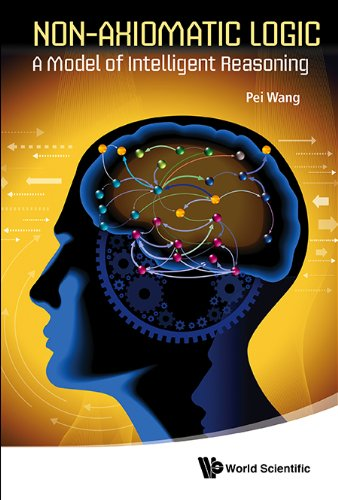
\includegraphics[scale=0.05]{figs/NAL.jpg} Non-Axiomatic Logic (NAL), \emph{Pei Wang, 2013}
  \item 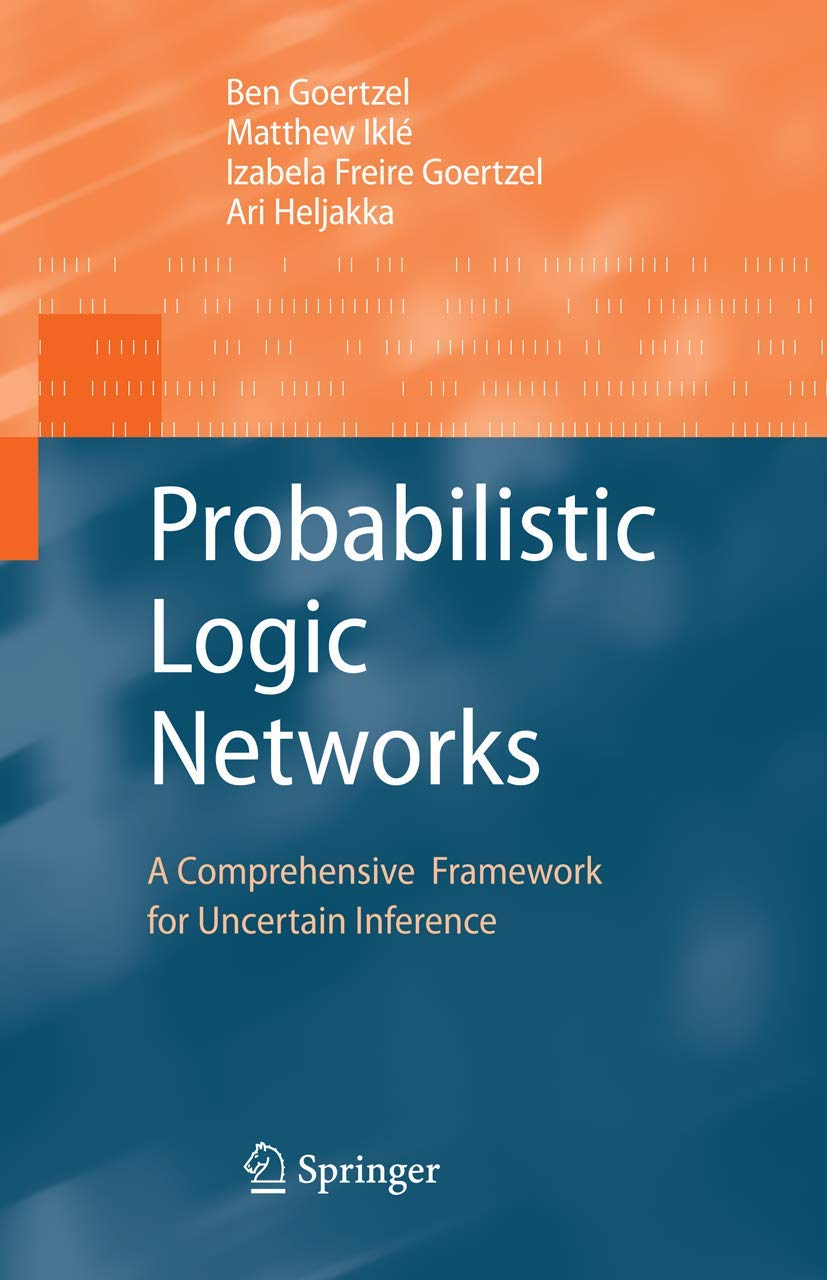
\includegraphics[scale=0.02]{figs/PLN.jpg} Probabilistic Logic Networks (PLN), \emph{Ben Goertzel et al, 2008}
  \item 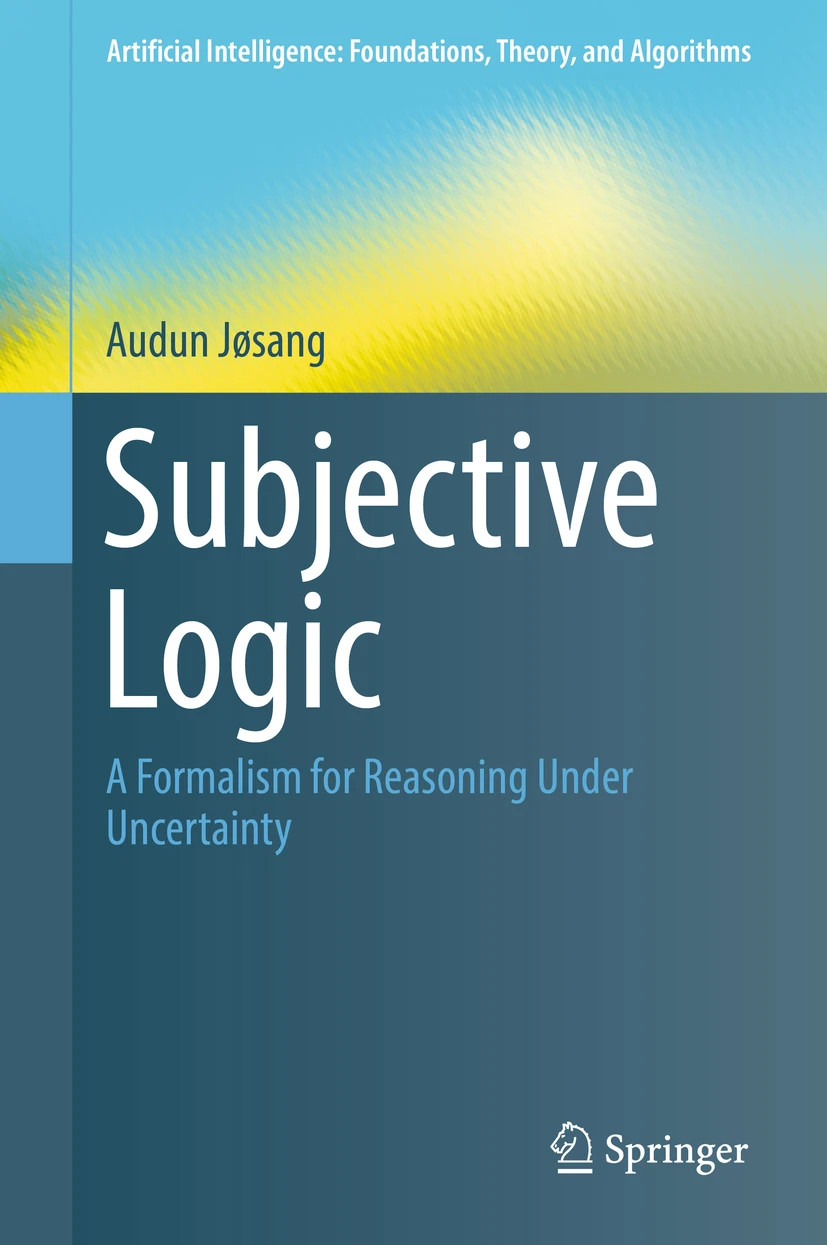
\includegraphics[scale=0.02]{figs/SL.jpg} Subjective Logic, \emph{Audun Jøsang, 2016}\\[1cm]
  \end{itemize}
  %% \begin{center}
  %% \digraph[scale=0.5]{fromtheorytotheorem}{
  %%     rankdir=LR;
  %%     node[shape=none, label=""] A;
  %%     node[shape=none, label=""] B;
  %%     A -> B [label=""];
  %% }
  %% \end{center}
  $$\rightarrow$$
  $$\Gamma\vdash\Tau$$
  $$\leftdasharrow$$
  %% \begin{center}
  %% \digraph[scale=0.5]{fromtheoremtotheory}{
  %%     rankdir=RL;
  %%     node[shape=none, label=""] A;
  %%     node[shape=none, label=""] B;
  %%     B -> A [style=dashed, label=""];
  %% }
  %% \end{center}
\end{frame}

\begin{frame}
  \frametitle{PLN Recall}
  \begin{columns}
    \column{5cm}
    \emph{\underline{Deduction:}}\\
    \digraph[scale=0.5]{deduction}{
      rankdir=LR;
      node[shape=none, label="A"] A;
      node[shape=none, label="B"] B;
      node[shape=none, label="C"] C;
      A -> B [label=""];
      B -> C [label=""];
      A -> C [style=dashed, label=""];
    }
    \begin{center}
      \begin{prooftree}
        \AxiomC{$B \limp C$}
        \AxiomC{$A \limp B$}
        \BinaryInfC{$A \limp C$}
      \end{prooftree}
    \end{center}
    \column{5cm}
    \pause
    \emph{\underline{Induction:}}\\
    \digraph[scale=0.5]{induction}{
      rankdir=LR;
      node[shape=none, label="A"] A;
      node[shape=none, label="B"] B;
      node[shape=none, label="C"] C;
      A -> B [label=""];
      B -> C [style=dashed, label=""];
      A -> C [label=""];
    }
    \begin{center}
      \begin{prooftree}
        \AxiomC{$A \limp C$}
        \AxiomC{$A \limp B$}
        \BinaryInfC{$B \limp C$}
      \end{prooftree}
    \end{center}
    \column{5cm}
    \pause
    \emph{\underline{Abduction:}}\\
    \digraph[scale=0.5]{abduction}{
      rankdir=LR;
      node[shape=none, label="A"] A;
      node[shape=none, label="B"] B;
      node[shape=none, label="C"] C;
      A -> B [style=dashed, label=""];
      B -> C [label=""];
      A -> C [label=""];
    }
    \begin{center}
      \begin{prooftree}
        \AxiomC{$A \limp C$}
        \AxiomC{$B \limp C$}
        \BinaryInfC{$A \limp B$}
      \end{prooftree}
    \end{center}
  \end{columns}
\end{frame}

\begin{frame}
  \frametitle{PLN Recall}
  \begin{columns}
    \column{5cm}
    \underline{\emph{Truth Value:}}
    $$A \limp B\ \measeq\ \texttt{TV}$$
    %% \begin{itemize}
  %% \item
    \begin{center}
      $\texttt{TV}$\\
      =\\
      \emph{Second Order Probability Distribution}
    \end{center}
    %% \end{itemize}
    \column{10cm}
    \only<1>{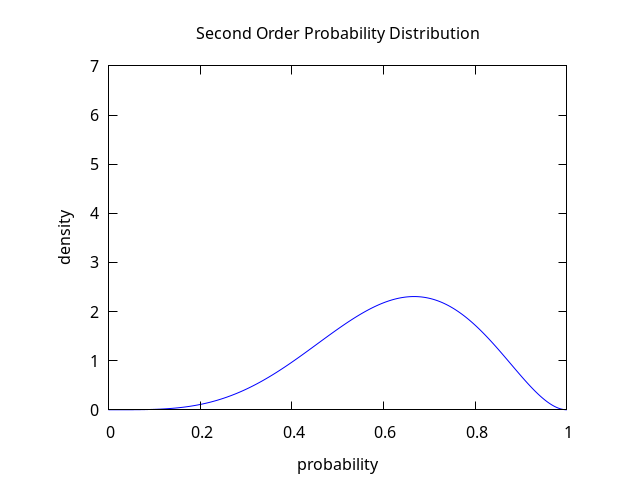
\includegraphics[scale=0.4]{figs/second_order.png}}
  \end{columns}
\end{frame}

\begin{frame}
  \frametitle{PLN Recall}
  \begin{columns}
    \column{5cm}
    \underline{\emph{Simple Truth Value:}}
    $$A \limp B\ \measeq\ \STV{s}{c}$$
    \begin{itemize}
    \item $s$ = \emph{strength}
    \item $c$ = \emph{confidence}
    \item Beta Distribution
    \end{itemize}
    \column{10cm}
    \only<1>{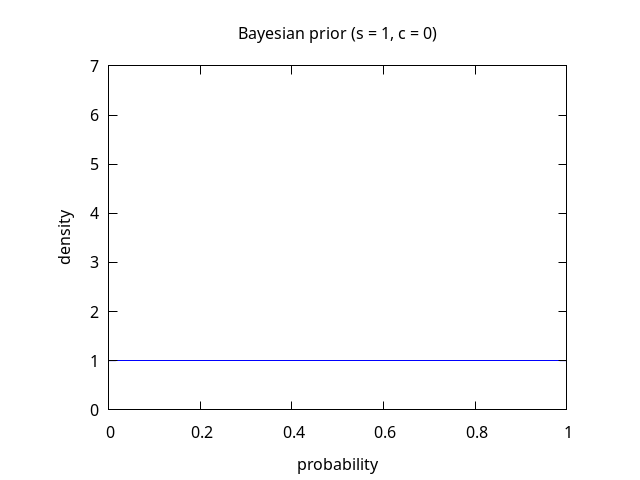
\includegraphics[scale=0.4]{figs/bayesian_prior.png}}%
    \only<2>{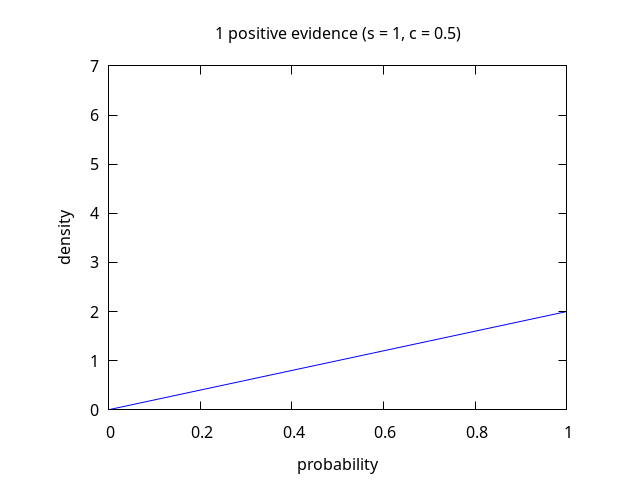
\includegraphics[scale=0.4]{figs/observations_0_1.png}}%
    \only<3>{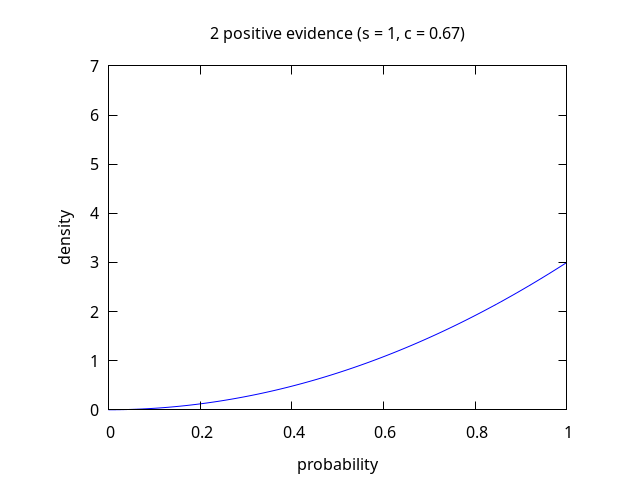
\includegraphics[scale=0.4]{figs/observations_0_2.png}}%
    \only<4>{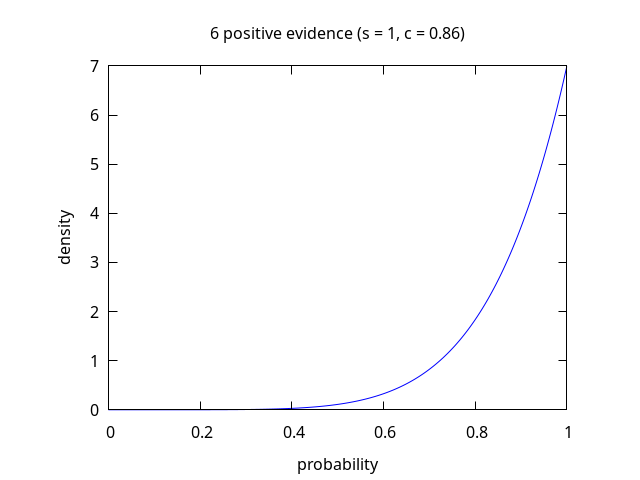
\includegraphics[scale=0.4]{figs/observations_0_6.png}}%
    \only<5>{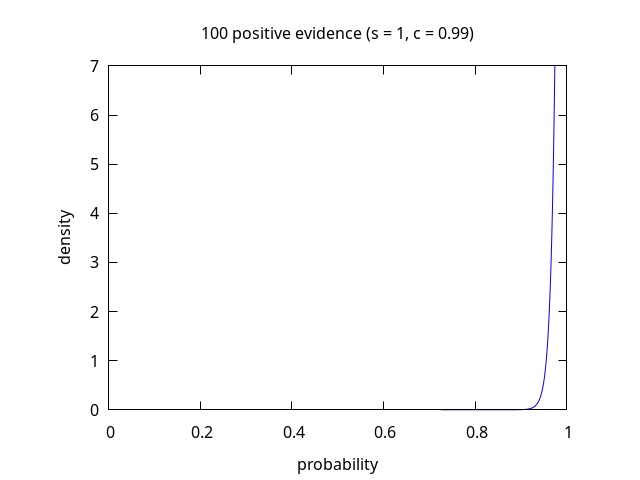
\includegraphics[scale=0.4]{figs/observations_0_100.png}}%
    \only<6>{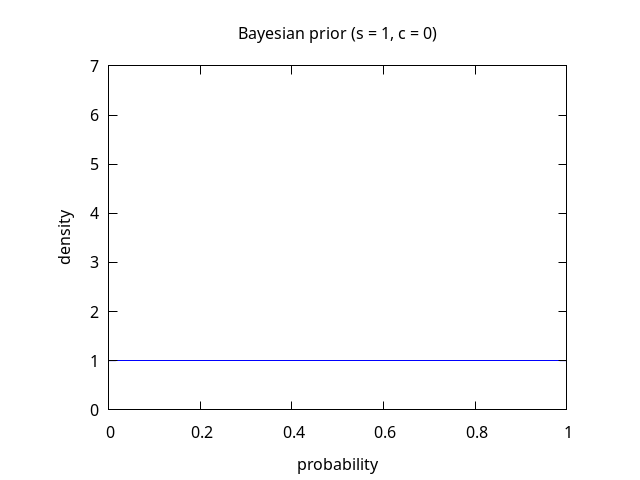
\includegraphics[scale=0.4]{figs/bayesian_prior.png}}%
    \only<7>{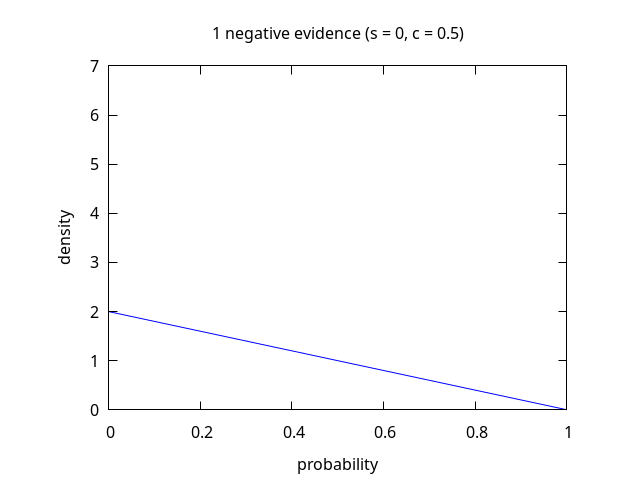
\includegraphics[scale=0.4]{figs/observations_1_0.png}}%
    \only<8>{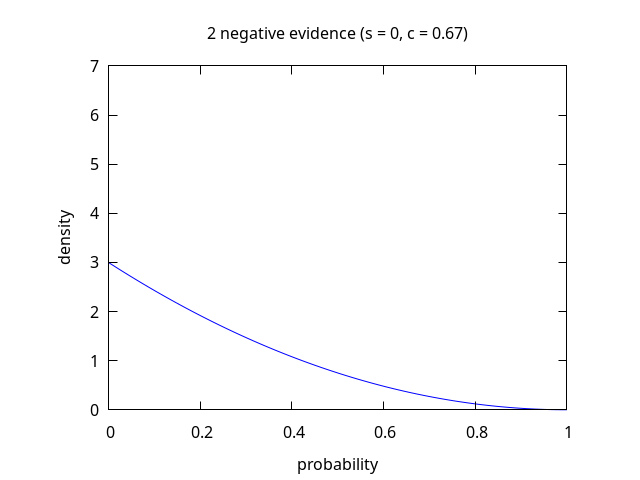
\includegraphics[scale=0.4]{figs/observations_2_0.png}}%
    \only<9>{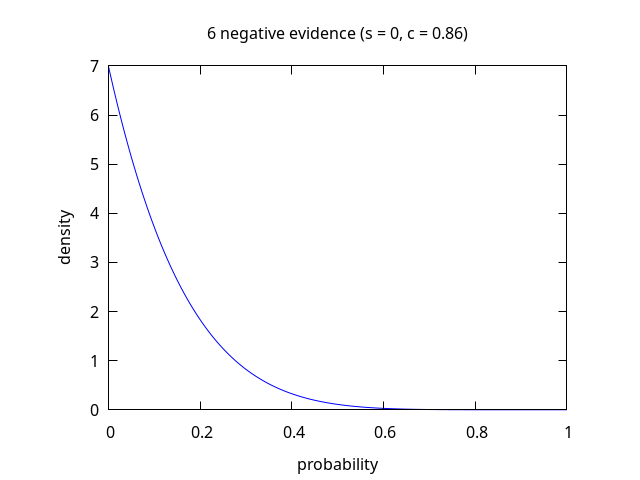
\includegraphics[scale=0.4]{figs/observations_6_0.png}}%
    \only<10>{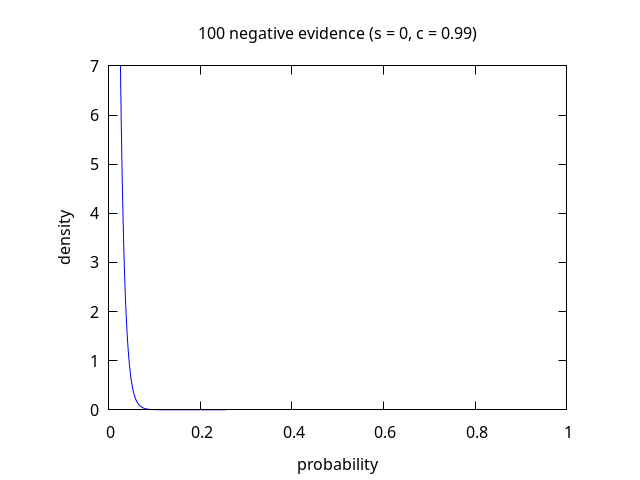
\includegraphics[scale=0.4]{figs/observations_100_0.png}}%
    \only<11>{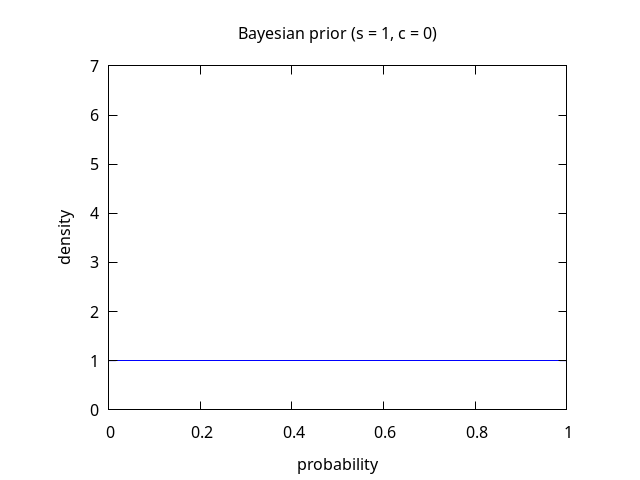
\includegraphics[scale=0.4]{figs/bayesian_prior.png}}%
    \only<12>{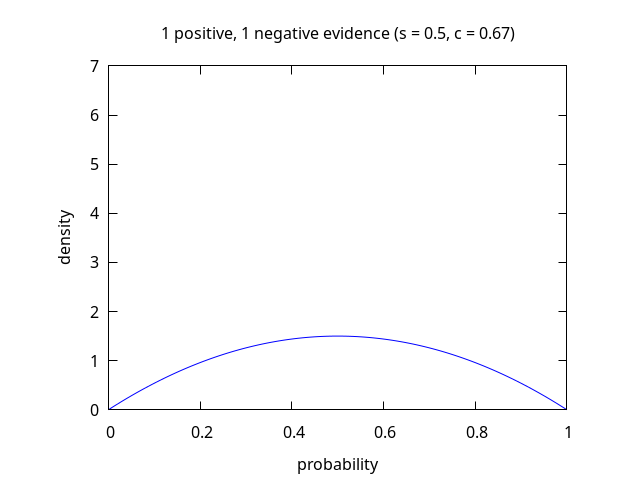
\includegraphics[scale=0.4]{figs/observations_1_1.png}}%
    \only<13>{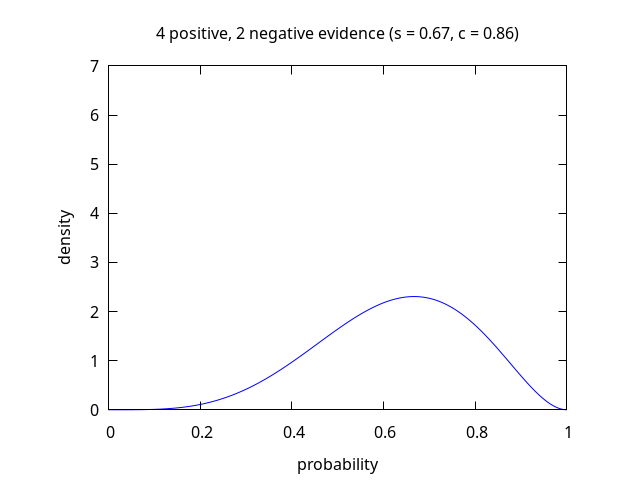
\includegraphics[scale=0.4]{figs/observations_2_4.png}}%
    \only<14>{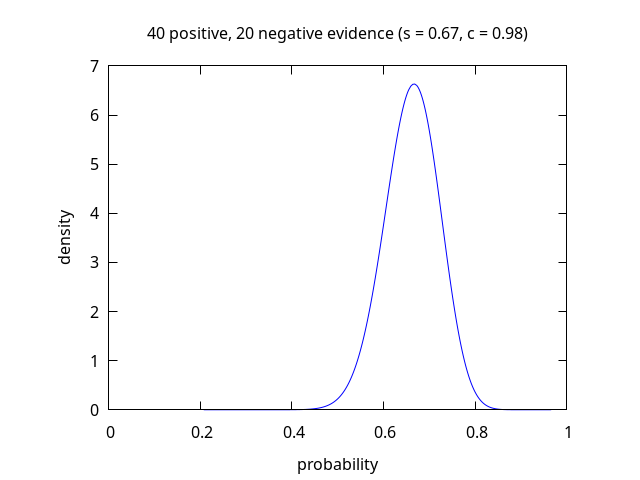
\includegraphics[scale=0.4]{figs/observations_20_40.png}}%
  \end{columns}
\end{frame}

\begin{frame}
  \frametitle{PLN Recall}
  \begin{columns}
    \column{7cm}
    \emph{\underline{Revision:}}\\
    \digraph[scale=0.5]{revision}{
      rankdir=LR;
      node[shape=none, label="A"] A;
      node[shape=none, label="B"] B;
      A -> B [label=""];
      A -> B [style=dashed, label=""];
      A -> B [label=""];
    }
    \begin{prooftree}
      \AxiomC{}
      \RightLabel{($e$)}
      \UnaryInfC{$A \limp B$}
      \AxiomC{}
      \RightLabel{($f$)}
      \UnaryInfC{$A \limp B$}
      \AxiomC{$e \perp f$}
      %% \RightLabel{($\text{R},e,f$)}
      \TrinaryInfC{$A \limp B$}
    \end{prooftree}
    \column{7cm}
    \begin{center}
      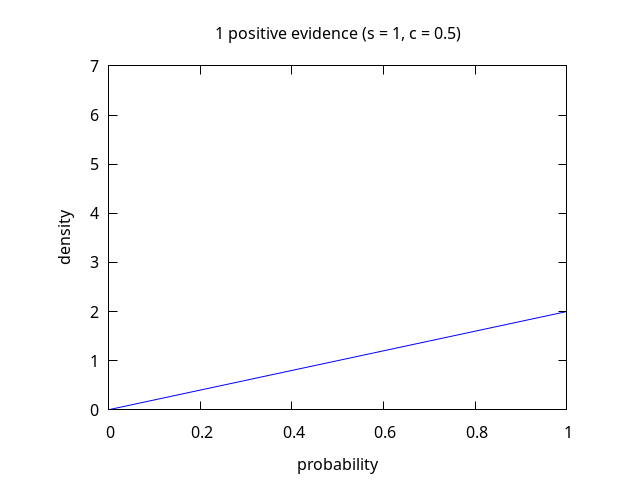
\includegraphics[scale=0.15]{figs/observations_0_1.png}
      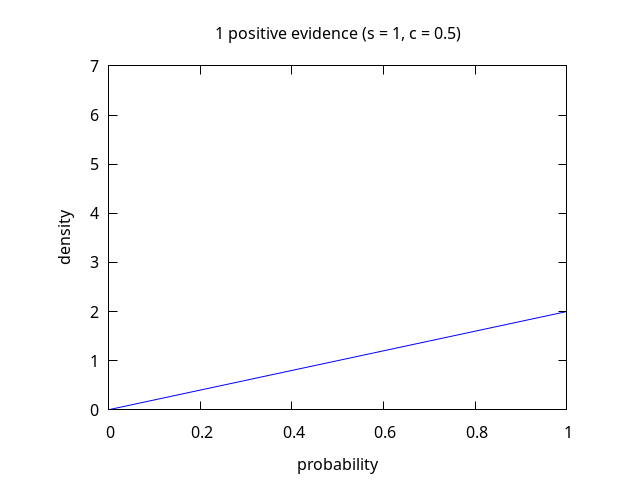
\includegraphics[scale=0.15]{figs/observations_0_1.png}
    \end{center}
    \begin{center}
      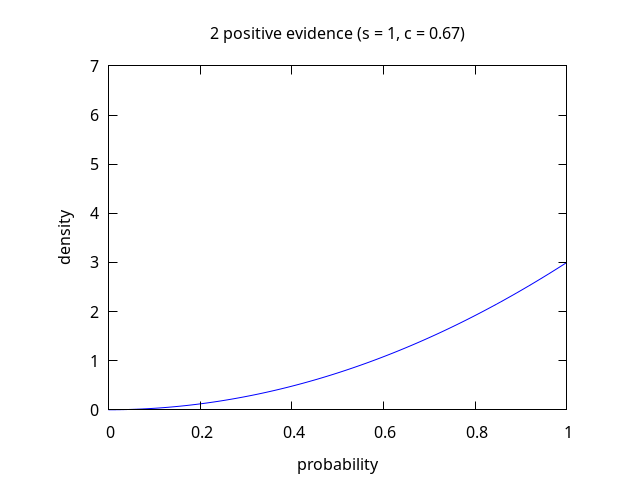
\includegraphics[scale=0.2]{figs/observations_0_2.png}
    \end{center}
  \end{columns}
\end{frame}

\begin{frame}
  \frametitle{PLN Recall}
  \begin{columns}
    \column{5cm}
    \emph{\underline{Induction + Revision:}}\\
    \digraph[scale=0.4]{multiinduction}{
      rankdir=LR;
      node[shape=none, label="A₁"] A1;
      node[shape=none, label="A₂"] A2;
      node[shape=none, label="A₃"] A3;
      node[shape=none, label="A₄"] A4;
      node[shape=none, label="B"] B;
      node[shape=none, label="C"] C;
      A1 -> B [label=""];
      A2 -> B [label=""];
      A3 -> B [label=""];
      A4 -> B [label=""];
      B -> C [style=dashed, label=""];
      A1 -> C [label=""];
      A2 -> C [label=""];
      A3 -> C [label=""];
      A4 -> C [label=""];
    }\\
    \column{10cm}
    \begin{center}
      \only<1>{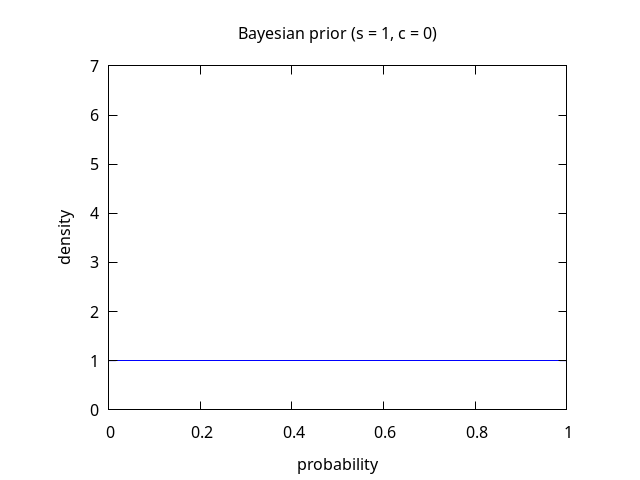
\includegraphics[scale=0.25]{figs/bayesian_prior.png}}%
      \only<2>{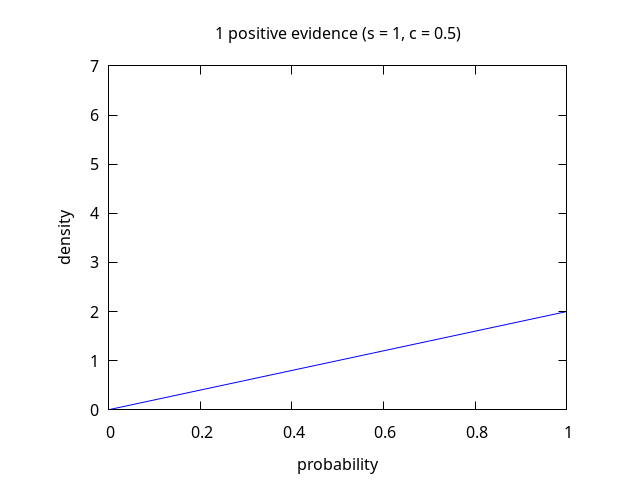
\includegraphics[scale=0.25]{figs/observations_0_1.png}}%
      \only<3>{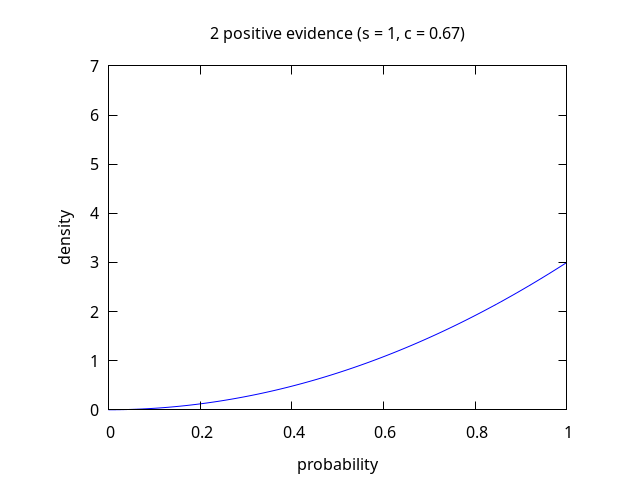
\includegraphics[scale=0.25]{figs/observations_0_2.png}}%
      \only<4>{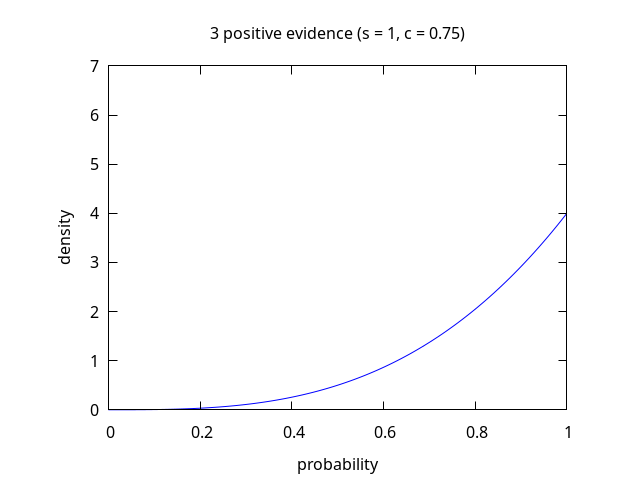
\includegraphics[scale=0.25]{figs/observations_0_3.png}}%
      \only<5>{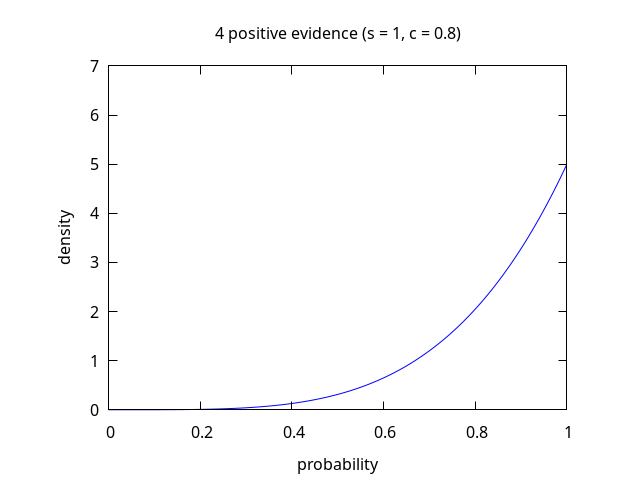
\includegraphics[scale=0.25]{figs/observations_0_4.png}}%
    \end{center}
  \end{columns}
      {\tiny
        \begin{prooftree}
          \AxiomC{{\color<2->{blue}$A_1 \limp C$}}
          \AxiomC{{\color<2->{blue}$A_1 \limp B$}}
          \RightLabel{{\color<2->{blue}(\Induction)}}
          \BinaryInfC{{\color<2->{blue}$B \limp C$}}
          \AxiomC{{\color<3->{blue}$A_2 \limp C$}}
          \AxiomC{{\color<3->{blue}$A_2 \limp B$}}
          \RightLabel{{\color<3->{blue}(\Induction)}}
          \BinaryInfC{{\color<3->{blue}$B \limp C$}}
          \RightLabel{{\color<3->{blue}(\Revision)}}
          \BinaryInfC{{\color<3->{blue}$B \limp C$}}
          \AxiomC{{\color<4->{blue}$A_3 \limp C$}}
          \AxiomC{{\color<4->{blue}$A_3 \limp B$}}
          \RightLabel{{\color<4->{blue}(\Induction)}}
          \BinaryInfC{{\color<4->{blue}$B \limp C$}}
          \RightLabel{{\color<4->{blue}(\Revision)}}
          \BinaryInfC{{\color<4->{blue}$B \limp C$}}
          \AxiomC{{\color<5->{blue}$A_4 \limp C$}}
          \AxiomC{{\color<5->{blue}$A_4 \limp B$}}
          \RightLabel{{\color<5->{blue}(\Induction)}}
          \BinaryInfC{{\color<5->{blue}$B \limp C$}}
          \RightLabel{{\color<5->{blue}(\Revision)}}
          \BinaryInfC{{\color<5->{blue}$B \limp C$}}
        \end{prooftree}
      }
\end{frame}

\begin{comment}
\begin{frame}
  \frametitle{PLN Recall}
  \emph{\underline{Induction + Revision:}}\\
       {\tiny
         \begin{prooftree}
           \AxiomC{$A_1 \limp C$}
           \AxiomC{$A_1 \limp B$}
           \RightLabel{(\Induction$,e$)}
           \BinaryInfC{$B \limp C\ \measeq\ \STV{1}{0.5}$}
           \AxiomC{$A_2 \limp C$}
           \AxiomC{$A_2 \limp B$}
           \RightLabel{(\Induction$,f$)}
           \BinaryInfC{$B \limp C\ \measeq\ \STV{1}{0.5}$}
           \AxiomC{$e \perp f$}
           \RightLabel{(\Revision$,e, f$)}
           \TrinaryInfC{$B \limp C\ \measeq\ \STV{1}{0.67}$}
           \AxiomC{$A_3 \limp C$}
           \AxiomC{$A_3 \limp B$}
           \RightLabel{(\Induction,$g$)}
           \BinaryInfC{$B \limp C\ \measeq\ \STV{1}{0.5}$}
           \AxiomC{$e,f \perp g$}
           \RightLabel{(\Revision$,e, f, g$)}
           \TrinaryInfC{$B \limp C\ \measeq\ \STV{1}{0.75}$}
         \end{prooftree}
       }
\end{frame}
\end{comment}

\begin{frame}
  \frametitle{PLN Recall}
  \begin{columns}
    \column{5cm}
    \underline{\emph{Induction + Revision example:}}
    \digraph[scale=0.4]{inductionexample}{
      rankdir=LR;
      node[shape=none, label="Tweety"] Tweety;
      node[shape=none, label="Sparrow"] Sparrow;
      node[shape=none, label="Doki"] Doki;
      node[shape=none, label="Goldie"] Goldie;
      node[shape=none, label="Bird"] Bird;
      node[shape=none, label="Fly"] Fly;
      Tweety -> Bird [label=""];
      Sparrow -> Bird [label=""];
      Doki -> Bird [label=""];
      Goldie -> Bird [label=""];
      Bird -> Fly [style=dashed, label=""];
      Tweety -> Fly [label=""];
      Sparrow -> Fly [label=""];
      Doki -> Fly [style=dotted, label=""];
      Goldie -> Fly [label=""];
    }\\
    \column{10cm}
    \begin{center}
      \only<1>{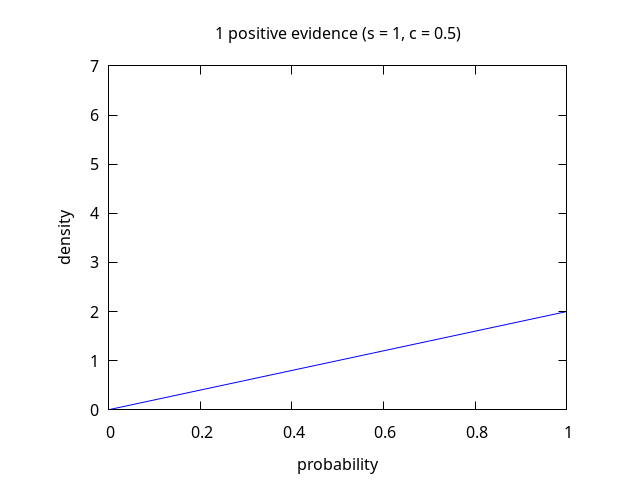
\includegraphics[scale=0.28]{figs/observations_0_1.png}}%
      \only<2>{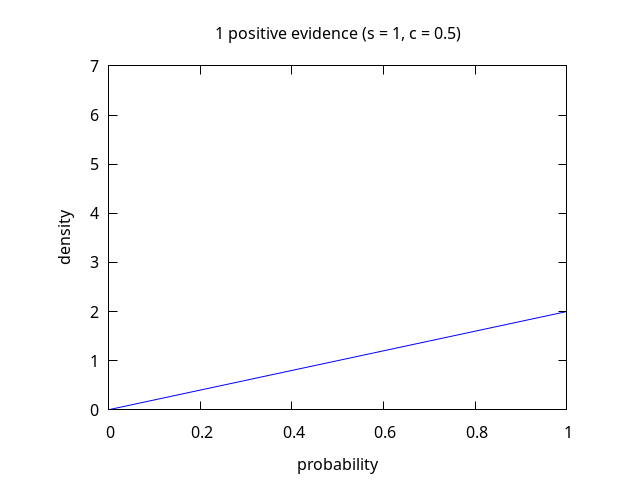
\includegraphics[scale=0.28]{figs/observations_0_1.png}}%
      \only<3>{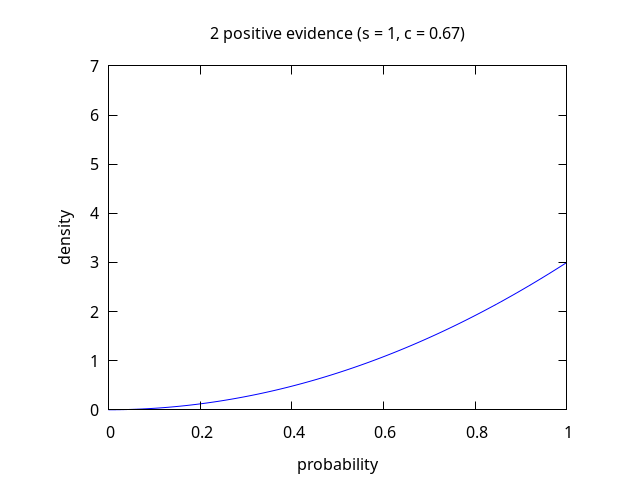
\includegraphics[scale=0.28]{figs/observations_0_2.png}}%
      \only<4>{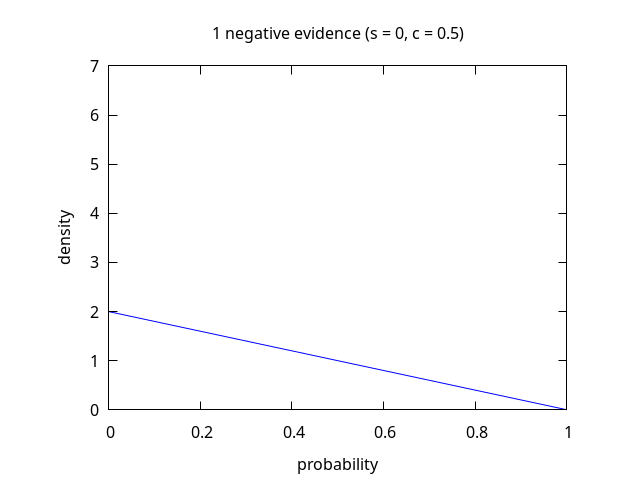
\includegraphics[scale=0.28]{figs/observations_1_0.png}}%
      \only<5>{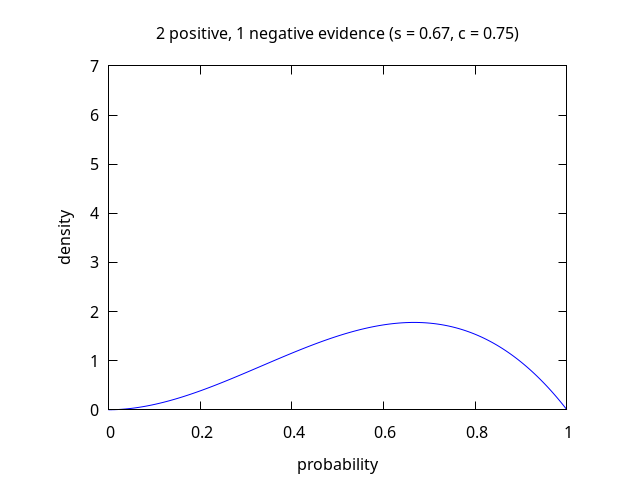
\includegraphics[scale=0.28]{figs/observations_1_2.png}}%
      \only<6>{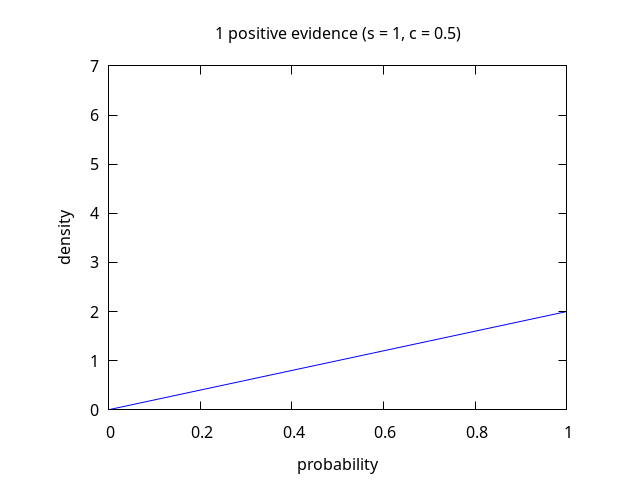
\includegraphics[scale=0.28]{figs/observations_0_1.png}}%
      \only<7>{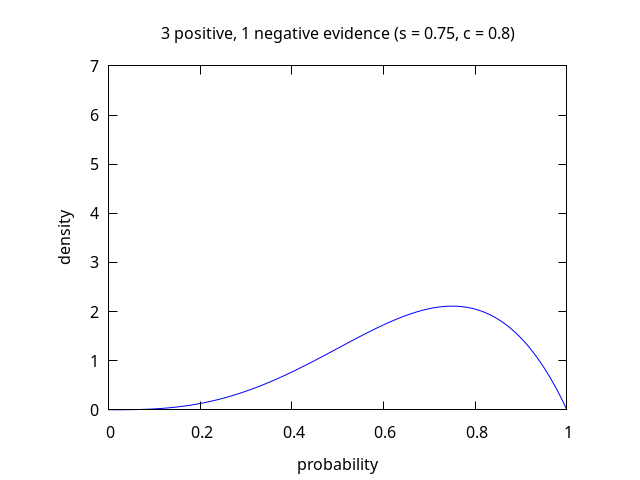
\includegraphics[scale=0.28]{figs/observations_1_3.png}}%
    \end{center}
  \end{columns}
  \vspace{0.2cm}
  \only<1>{
    {\footnotesize
      \begin{prooftree}
        \AxiomC{$\text{Tweety} \limp \text{Fly}\ \measeq\ \STV{1}{1}$}
        \AxiomC{$\text{Tweety} \limp \text{Bird}\ \measeq\ \STV{1}{1}$}
        \RightLabel{(\Induction$,t$)}
        \BinaryInfC{$\text{Bird} \limp \text{Fly}\ \measeq\ \STV{1}{0.5}$}
      \end{prooftree}
    }
  }
  \only<2>{
    {\footnotesize
      \begin{prooftree}
        \AxiomC{$\text{Sparrow} \limp \text{Fly}\ \measeq\ \STV{1}{1}$}
        \AxiomC{$\text{Sparrow} \limp \text{Bird}\ \measeq\ \STV{1}{1}$}
        \RightLabel{(\Induction$,s$)}
        \BinaryInfC{$\text{Bird} \limp \text{Fly}\ \measeq\ \STV{1}{0.5}$}
      \end{prooftree}
    }
  }
  \only<3>{
    {\footnotesize
      \begin{prooftree}
        \AxiomC{}
        \RightLabel{(t)}
        \UnaryInfC{$\text{Bird} \limp \text{Fly}\ \measeq\ \STV{1}{0.5}$}
        \AxiomC{}
        \RightLabel{(s)}
        \UnaryInfC{$\text{Bird} \limp \text{Fly}\ \measeq\ \STV{1}{0.5}$}
        \AxiomC{$t \perp s$}
        \RightLabel{(\Revision$,t,s$)}
        \TrinaryInfC{$\text{Bird} \limp \text{Fly}\ \measeq\ \STV{1}{0.67}$}
      \end{prooftree}
    }
  }
  \only<4>{
    {\footnotesize
      \begin{prooftree}
        \AxiomC{$\text{Doki} \limp \text{Fly}\ \measeq\ \STV{0}{1}$}
        \AxiomC{$\text{Doki} \limp \text{Bird}\ \measeq\ \STV{1}{1}$}
        \RightLabel{(\Induction$,d$)}
        \BinaryInfC{$\text{Bird} \limp \text{Fly}\ \measeq\ \STV{0}{0.5}$}
      \end{prooftree}
    }
  }
  \only<5>{
    {\footnotesize
      \begin{prooftree}
        \AxiomC{}
        \RightLabel{(t,s)}
        \UnaryInfC{$\text{Bird} \limp \text{Fly}\ \measeq\ \STV{1}{0.67}$}
        \AxiomC{}
        \RightLabel{(d)}
        \UnaryInfC{$\text{Bird} \limp \text{Fly}\ \measeq\ \STV{0}{0.5}$}
        \AxiomC{$t,s \perp d$}
        \RightLabel{(\Revision$,t,s,d$)}
        \TrinaryInfC{$\text{Bird} \limp \text{Fly}\ \measeq\ \STV{0.67}{0.75}$}
      \end{prooftree}
    }
  }
  \only<6>{
    {\footnotesize
      \begin{prooftree}
        \AxiomC{$\text{Goldie} \limp \text{Fly}\ \measeq\ \STV{1}{1}$}
        \AxiomC{$\text{Goldie} \limp \text{Bird}\ \measeq\ \STV{1}{1}$}
        \RightLabel{(\Induction$,g$)}
        \BinaryInfC{$\text{Bird} \limp \text{Fly}\ \measeq\ \STV{1}{0.5}$}
      \end{prooftree}
    }
  }
  \only<7>{
    {\footnotesize
      \begin{prooftree}
        \AxiomC{}
        \RightLabel{(t,s,d)}
        \UnaryInfC{$\text{Bird} \limp \text{Fly}\ \measeq\ \STV{0.67}{0.75}$}
        \AxiomC{}
        \RightLabel{(g)}
        \UnaryInfC{$\text{Bird} \limp \text{Fly}\ \measeq\ \STV{1}{0.5}$}
        \AxiomC{$t,s,d \perp g$}
        \RightLabel{(\Revision$,t,s,d,g$)}
        \TrinaryInfC{$\text{Bird} \limp \text{Fly}\ \measeq\ \STV{0.75}{0.8}$}
      \end{prooftree}
    }
  }
  \vspace{0.8cm}
\end{frame}

\begin{frame}
  \frametitle{PLN Recall}
  \begin{columns}
    \column{7cm}
    \underline{\emph{Abduction + Revision:}}\\
    \vspace{0.2cm}
    \digraph[scale=0.4]{abductionexample}{
      rankdir=LR;
      node[shape=none, label="Bird"] Bird;
      node[shape=none, label="Fly"] Fly;
      node[shape=none, label="Aerodynamic"] Aerodynamic;
      node[shape=none, label="HasFeather"] HasFeather;
      node[shape=none, label="HasWing"] HasWing;
      node[shape=none, label="ConsumeEnergy"] ConsumeEnergy;
      Bird -> Fly [style=dashed, label=""];
      Bird -> Aerodynamic [label=""];
      Bird -> HasFeather [label=""];
      Bird -> HasWing [label=""];
      Bird -> ConsumeEnergy [label=""];
      Fly -> Aerodynamic [label=""];
      Fly -> HasWing [label=""];
      Fly -> HasFeather [style=dotted, label=""];
      Fly -> ConsumeEnergy [label=""];
    }
    \vspace{0.4cm}
    %% \pause
    \column{7cm}
    \underline{\emph{Induction + Abduction + Revision:}}\\
    \vspace{0.2cm}
    \digraph[scale=0.4]{inductionabductionexample}{
      rankdir=LR;
      node[shape=none, label="Tweety"] Tweety;
      node[shape=none, label="Sparrow"] Sparrow;
      node[shape=none, label="Doki"] Doki;
      node[shape=none, label="Goldie"] Goldie;
      node[shape=none, label="Bird"] Bird;
      node[shape=none, label="Fly"] Fly;
      node[shape=none, label="Aerodynamic"] Aerodynamic;
      node[shape=none, label="HasFeather"] HasFeather;
      node[shape=none, label="HasWing"] HasWing;
      node[shape=none, label="ConsumeEnergy"] ConsumeEnergy;
      Tweety -> Bird [label=""];
      Sparrow -> Bird [label=""];
      Doki -> Bird [label=""];
      Goldie -> Bird [label=""];
      Tweety -> Fly [label=""];
      Sparrow -> Fly [label=""];
      Doki -> Fly [style=dotted, label=""];
      Goldie -> Fly [label=""];
      Bird -> Fly [style=dashed, label=""];
      Bird -> Aerodynamic [label=""];
      Bird -> HasFeather [label=""];
      Bird -> HasWing [label=""];
      Bird -> ConsumeEnergy [label=""];
      Fly -> Aerodynamic [label=""];
      Fly -> HasWing [label=""];
      Fly -> HasFeather [style=dotted, label=""];
      Fly -> ConsumeEnergy [label=""];
    }
    %% \vspace{0.6cm}
  \end{columns}
  %% \pause
  PLN also has:
  \begin{itemize}
  \item Quantifiers $\exists$, $\forall$
  \item Traditional Connectors $\land$, $\lor$, $\neg$
  \item Probabilistic Computational Model
  \end{itemize}
\end{frame}

\begin{frame}
  \frametitle{PLN and Theorem Proving}
  Crisp Reasoning
\end{frame}

\begin{frame}
  \frametitle{PLN and Theorem Proving}
  \begin{columns}
    \column{7cm}
    \only<2->{
    \underline{\emph{Induction + Revision:}}\\
    \digraph[scale=0.4]{inductiontheo}{
      rankdir=LR;
      node[shape=none, label="T₁"] T1;
      node[shape=none, label="T₂"] T2;
      node[shape=none, label="T₃"] T3;
      node[shape=none, label="T₄"] T4;
      node[shape=none, label="T₅"] T5;
      node[shape=none, label="..."] T6;
      node[shape=none, label="H"] H;
      node[shape=none, label="C"] C;
      T1 -> H [label=""];
      T2 -> H [label=""];
      T3 -> H [label=""];
      T4 -> H [label=""];
      T5 -> H [label=""];
      T6 -> H [label=""];
      H -> C [style=dashed, label=""];
      T1 -> C [label=""];
      T2 -> C [label=""];
      T3 -> C [label=""];
      T4 -> C [label=""];
      T5 -> C [label=""];
      T6 -> C [label=""];
    }}
    \column{7cm}
    \only<3->{
    \underline{\emph{Abduction + Revision:}}\\
    \digraph[scale=0.4]{abductionforall}{
      rankdir=LR;
      node[shape=none, label="T"] T;
      node[shape=none, label="∀x P(x)"] ForAll;
      node[shape=none, label="P(0)"] P0;
      node[shape=none, label="P(1)"] P1;
      node[shape=none, label="P(2)"] P2;
      node[shape=none, label="P(3)"] P3;
      node[shape=none, label="P(4)"] P4;
      node[shape=none, label="..."] P5;
      T -> ForAll [style=dashed, label=""];
      T -> P0 [label=""];
      T -> P1 [label=""];
      T -> P2 [label=""];
      T -> P3 [label=""];
      T -> P4 [label=""];
      T -> P5 [label=""];
      ForAll -> P0 [label=""];
      ForAll -> P1 [label=""];
      ForAll -> P2 [label=""];
      ForAll -> P3 [label=""];
      ForAll -> P4 [label=""];
      ForAll -> P5 [label=""];
    }}
  \end{columns}
  $$\phi \vdash_{\Gamma} \psi\ :=\ \exists p\ \Theta(\Gamma, p, \phi)\ \limp\ \exists q\ \Theta(\Gamma, q, \psi)$$
  \only<1>{
    \begin{center}
    \digraph[scale=0.5]{entail}{
      rankdir=LR;
      node[shape=none, label="𝜙"] phi;
      node[shape=none, label="𝜓"] psi;
      phi -> psi [label=""];
    }
    \end{center}
  }
\end{frame}

\begin{frame}
  \begin{center}
  Time for demo
  \end{center}
\end{frame}

\begin{frame}
  \frametitle{Conclusion}

  \begin{itemize}
  \item Glorified memoizer
  \item Discover patterns with induction and abduction
  \end{itemize}
\end{frame}

\end{document}
